% HEADER
\documentclass[class=article, crop=false]{standalone}
\usepackage{00_Preamble/frr_preamble}

% Packages
\usepackage{titlesec}
\usepackage{hyperref}
\usepackage{float}
\usepackage{graphics}
\usepackage{placeins}
\usepackage{adjustbox}
% END HEADER

\begin{document}
	\subsection{Final Design}
	\label{subsec:final-design}
	
	After the preliminary design was completed, several design iterations were made as the CAD assembly was further developed and specific parts were selected. Changes were made to resolve size constraint issues, reduce fabrication time, and reduce system cost. The final CAD assembly of the robot is presented in Figure \ref{fig:final-cad}.
	
	\FloatBarrier
	\begin{figure}[h]
	\centering
	 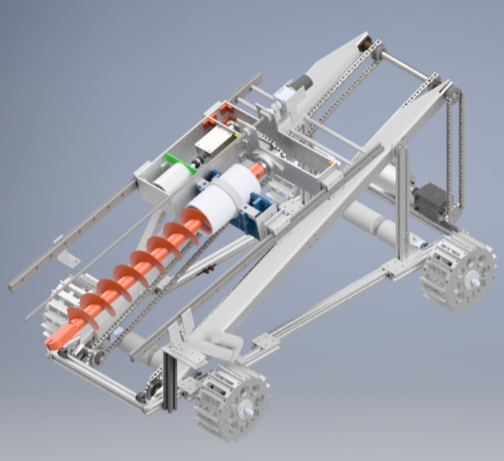
\includegraphics[width=0.45\linewidth]{09_Figures/final-cad.jpg}
	 \caption{Final Robot CAD Assembly}
	 \label{fig:final-cad}
	\end{figure}
	\FloatBarrier
	
	\subsubsection{Frame Section}
	
	The frame was designed to be lightweight and simple to modify (Figure \ref{fig:frame-cad}). It was constructed from 30mm by 30mm aluminum extrusions connected by corner brackets and flat mounting plates. Two vertical supports near the back connect the conveyor. The motor and gearbox that drive the conveyor were placed on the back extrusion. Only minor length changes were made to the frame between the preliminary design review and the final design. The final weight, excluding the wheels was under 4 kg.
	
	The wheel diameter was reduced to 7.875 inches since the rover was above the RMC height limit with the previous 30 cm diameter. The units were switched from metric to U.S. customary to aid in machining. The motor mount height was also decreased to lower the robot height.

	The final wheel design (Figure \ref{fig:wheel-cad}) was modified to be easier to fabricate. The first design had many components that would make assembly challenging and could lead to points of failure. The wheel rim was eliminated to decrease weight. It did not provide much structural support, as most of the load is distributed through the sides of the wheel. The grousers are press fit and bolted into the wheel sides instead of using 3D printed spacers. The number of grousers was increased from twelve to eighteen. This increases traction and smoothes the ride. 

	VEX CIM motors were chosen to drive the wheels. The motors provide a maximum of 337 Watts. VEX parts are easy to assemble, as all the parts interface well together. Hex shafts were used over rotary shafts to increase the torque transmission between the axles and the wheels.
	
	
	\begin{figure}
	\centering
	\begin{minipage}{.49\textwidth}
	  \centering
	  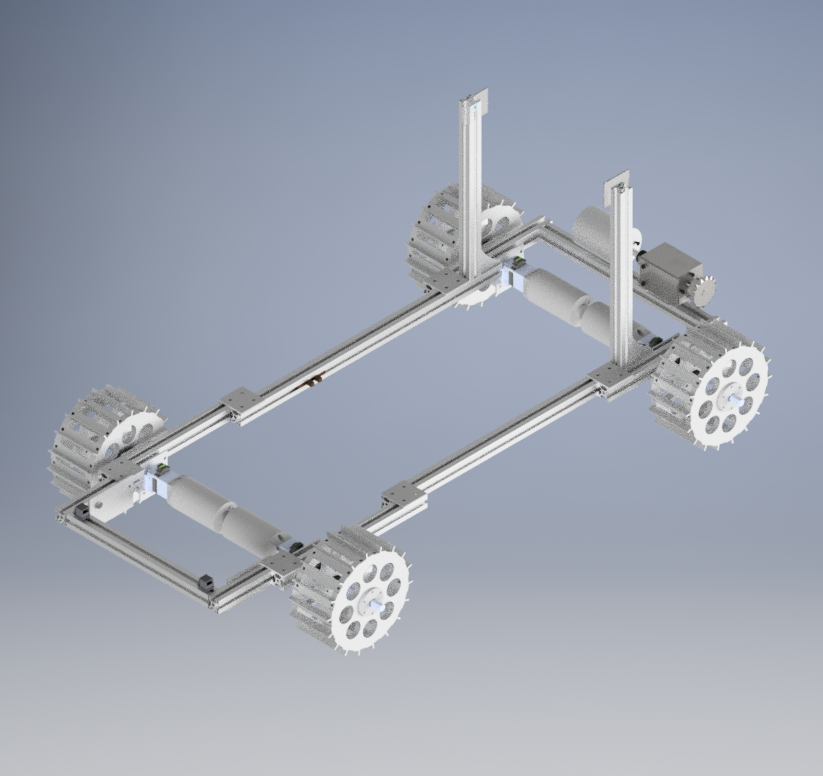
\includegraphics[width=.9\linewidth]{09_Figures/frame-cad.jpg}
	  \captionof{figure}{Final CAD Frame Assembly}
	  \label{fig:frame-cad}
	\end{minipage}
	\begin{minipage}{.49\textwidth}
	  \centering
	  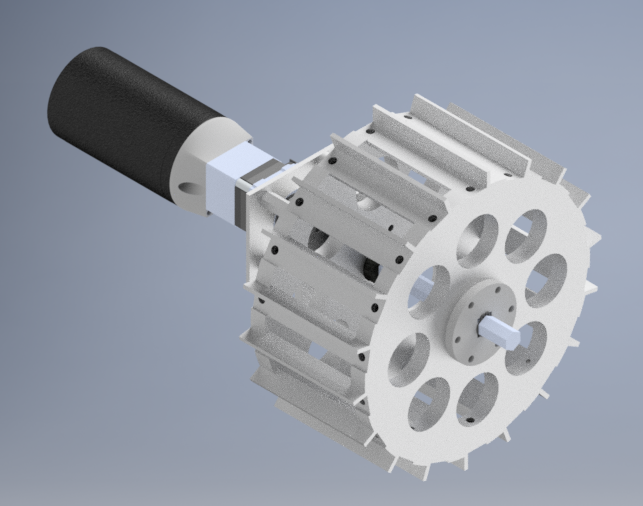
\includegraphics[width=.9\linewidth]{09_Figures/wheel-cad.jpg}
	  \captionof{figure}{Final Wheel Assembly}
	  \label{fig:wheel-cad}
	\end{minipage}
	\end{figure}
	
	
	\subsubsection{Excavation System}
	
	The auger must travel from its initial position to ground level during operation. The carriage, shown in Figure \ref{fig:carriage-cad}, supports the excavation system and contains the motor and gearbox that drive the auger. 
	
	A 2.2 horsepower motor and \#40 ANSI roller chain are used to drive the auger.  A flanged bushing and ball bearing support the auger from radial and thrust loads. Polycarbonate sheets cover the top and bottom of the carriage to protect the auger drive system from dust.
	
	The primary factors when selecting the auger were mass, digging length, power consumption, and ease of assembly. A 34 in. auger with a 4 in. radius was determined to travel deep enough to mine the icy gravel. 
	
	\begin{wrapfigure}{l}{0.5\textwidth}
	\centering
	 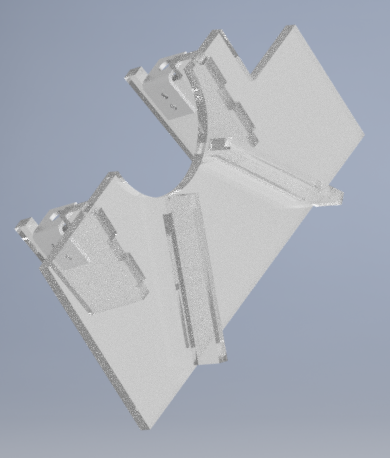
\includegraphics[width=0.4\textwidth]{09_Figures/fan-cad.jpg}
	 \caption{The Final Fan Assembly}
	 \label{fig:fan-cad}
	\end{wrapfigure}
	
	A PVC pipe was fitted to the auger to aid in regolith and gravel acquisition. The upward helical spiral on the auger funnels the gravel into the PVC pipe and can then be deposited into the collection bin. The tube is 8 in. long and has a 4.75 in. inner diameter and 5 in. outer diameter. 
	
	Due to size constraints, the auger must start the match constricted near the conveyor. Once the match begins, two linear actuators push the auger to its final angle of $75^\circ$ from the horizontal. A final angle of $60^{\circ}$ was desired, but it was not possible to fit an auger with the correct digging length at $60^\circ$ and fit within the RMC size constraints. The linear actuators and guide rails support the carriage as the auger travels to ground level. A lead screw driven by a motor provides the linear motion. The carriage and guide rails are attached directly to the frame.
	
	The fan is a system (Figure \ref{fig:fan-cad}) made of laser cut polycarbonate sheets that spreads out the icy regolith as it falls into the depositing system. This allows the material to be deposited evenly on the conveyor. Without the fan, the material would pile up in the center of the conveyor. 
	
	
	\subsubsection{Depositing}
	
	The gravel depositing system consists of a conveyor belt with standard \#40 ANSI roller chains and sprockets (Fig. XX). It was determined that three supports were needed along the 4 feet conveyor belt to prevent roller chain deflection. A hollow rod was used for the middle support to reduce weight. Tensioners were attached at the bottom of each roller chain to allow for variable tension in case the roller chain deflected under heavy gravel loads. Flanged bushings were chosen to support the radial load on the rods since they were easy to assemble. The conveyor is driven from the back rod by a roller chain that runs to the frame and is connected to a motor and gearbox. The drive shaft is keyed to couple the two roller chains together and prevent misalignment. 
	
	A nylon mesh was chosen as the conveyor belt so that BP-1 could be filtered out and no excess weight would be carried. The mesh is not shown in the CAD because it would be too computationally intensive to render.




	
	
	


	
\end{document}
